% !TeX root=main.tex

\chapter{ارزیابی روش پیشنهادی} \label{ch:eval}
\thispagestyle{empty}


\section{مقدمه}
\paragraph{}{
    در این فصل برای بررسی عملکرد روش پیشنهادی در فصل قبل، نرم‌افزار ارزیابی‌ای نوشته شده است که بدون دخالت کوبرنیتز امکان ارزیابیی سامانه را بما دهد.
    از آن‌جایی که این نمونه‌ای مشابه‌ای از این روش وجود ندارد فقط ارزیابی خود روش را قرار می‌دهیم.
    \\
    سخت‌افزار مورد تست یک دستگاه رزبری‌پای با مشخصات زیر می‌باشد:
    \begin{latin}
        \begin{lstlisting}{language=text}
    System Model: Raspberry Pi 4 Model B Rev 1.4
    Software Info:
        Operating System: GNU/Linux
        Distribution: Ubuntu
        Kernel: 5.15.0-1024-raspi
        Arch: aarch64(arm64)
    Hardware Info:
        CPU: 4
        Memory: 7.62502 GiB
        \end{lstlisting}
    \end{latin}
    \newpage
}

\section{
    بررسی توان تامین‌کننده با تعداد دستگاه‌های اینترنت اشیاء مختلف
}
\label{sec:different_devices}
\paragraph{}
{
    با توجه به اینکه تامین‌کننده از ترکیب قرارداد انتقال فرا متن و معماری فن‌آوت استفاده می‌کند،
    امکان پایش تعداد زیادی دستگاه‌ اینترنت اشیاء را دارد. حال به بررسی‌های انجام شده با استفاده از 
    نرم‌افزار ارزیابی می‌پردازیم، در این بررسی یک کنترل‌کننده وجود دارد و تعداد دستگاه‌ها متغییر است:
%     1,320.927926ms,"Controllers: 1, DevicesPerController: 1, Duration: 5s"
% 10,325.609733ms,"Controllers: 1, DevicesPerController: 10, Duration: 5s"
% 100,328.67701ms,"Controllers: 1, DevicesPerController: 100, Duration: 5s"
% 1000,332.549921ms,"Controllers: 1, DevicesPerController: 1000, Duration: 5s"
% 10000,403.699692ms,"Controllers: 1, DevicesPerController: 10000, Duration: 5s"
% 100000,1150.619205ms,"Controllers: 1, DevicesPerController: 100000, Duration: 5s"
    \begin{table}[h]
        \centering
        \begin{tabular}{|c|c|}
        \hline
            تعداد دستگاه & مدت زمان                                                                                  \\ \hline
            ۱     &   \lr{۳۲۰.۹۲۷} میلی ثانیه                    \\ \hline
            ۱۰     &   \lr{۳۲۸.۶۷۷} میلی ثانیه                      \\ \hline
            ۱۰۰     &  \lr{۳۲۵۰.۶۰۹} میلی ثانیه                    \\ \hline
            ۱۰۰۰     &  \lr{۳۳۲.۵۴۹} میلی ثانیه                                                              \\ \hline
            ۱۰۰۰۰     & \lr{۴۰۲.۶۹۹} میلی ثانیه                  \\ \hline
            ۱۰۰۰۰۰     & \lr{۱۱۵۰.۶۱۹} میلی ثانیه  \\ \hline
        \end{tabular}
        \caption{جدول تعداد دستگاه‌ها به مدت زمان}
        \label{different_devices_table}
    \end{table}

    \begin{figure}[H]
        \center{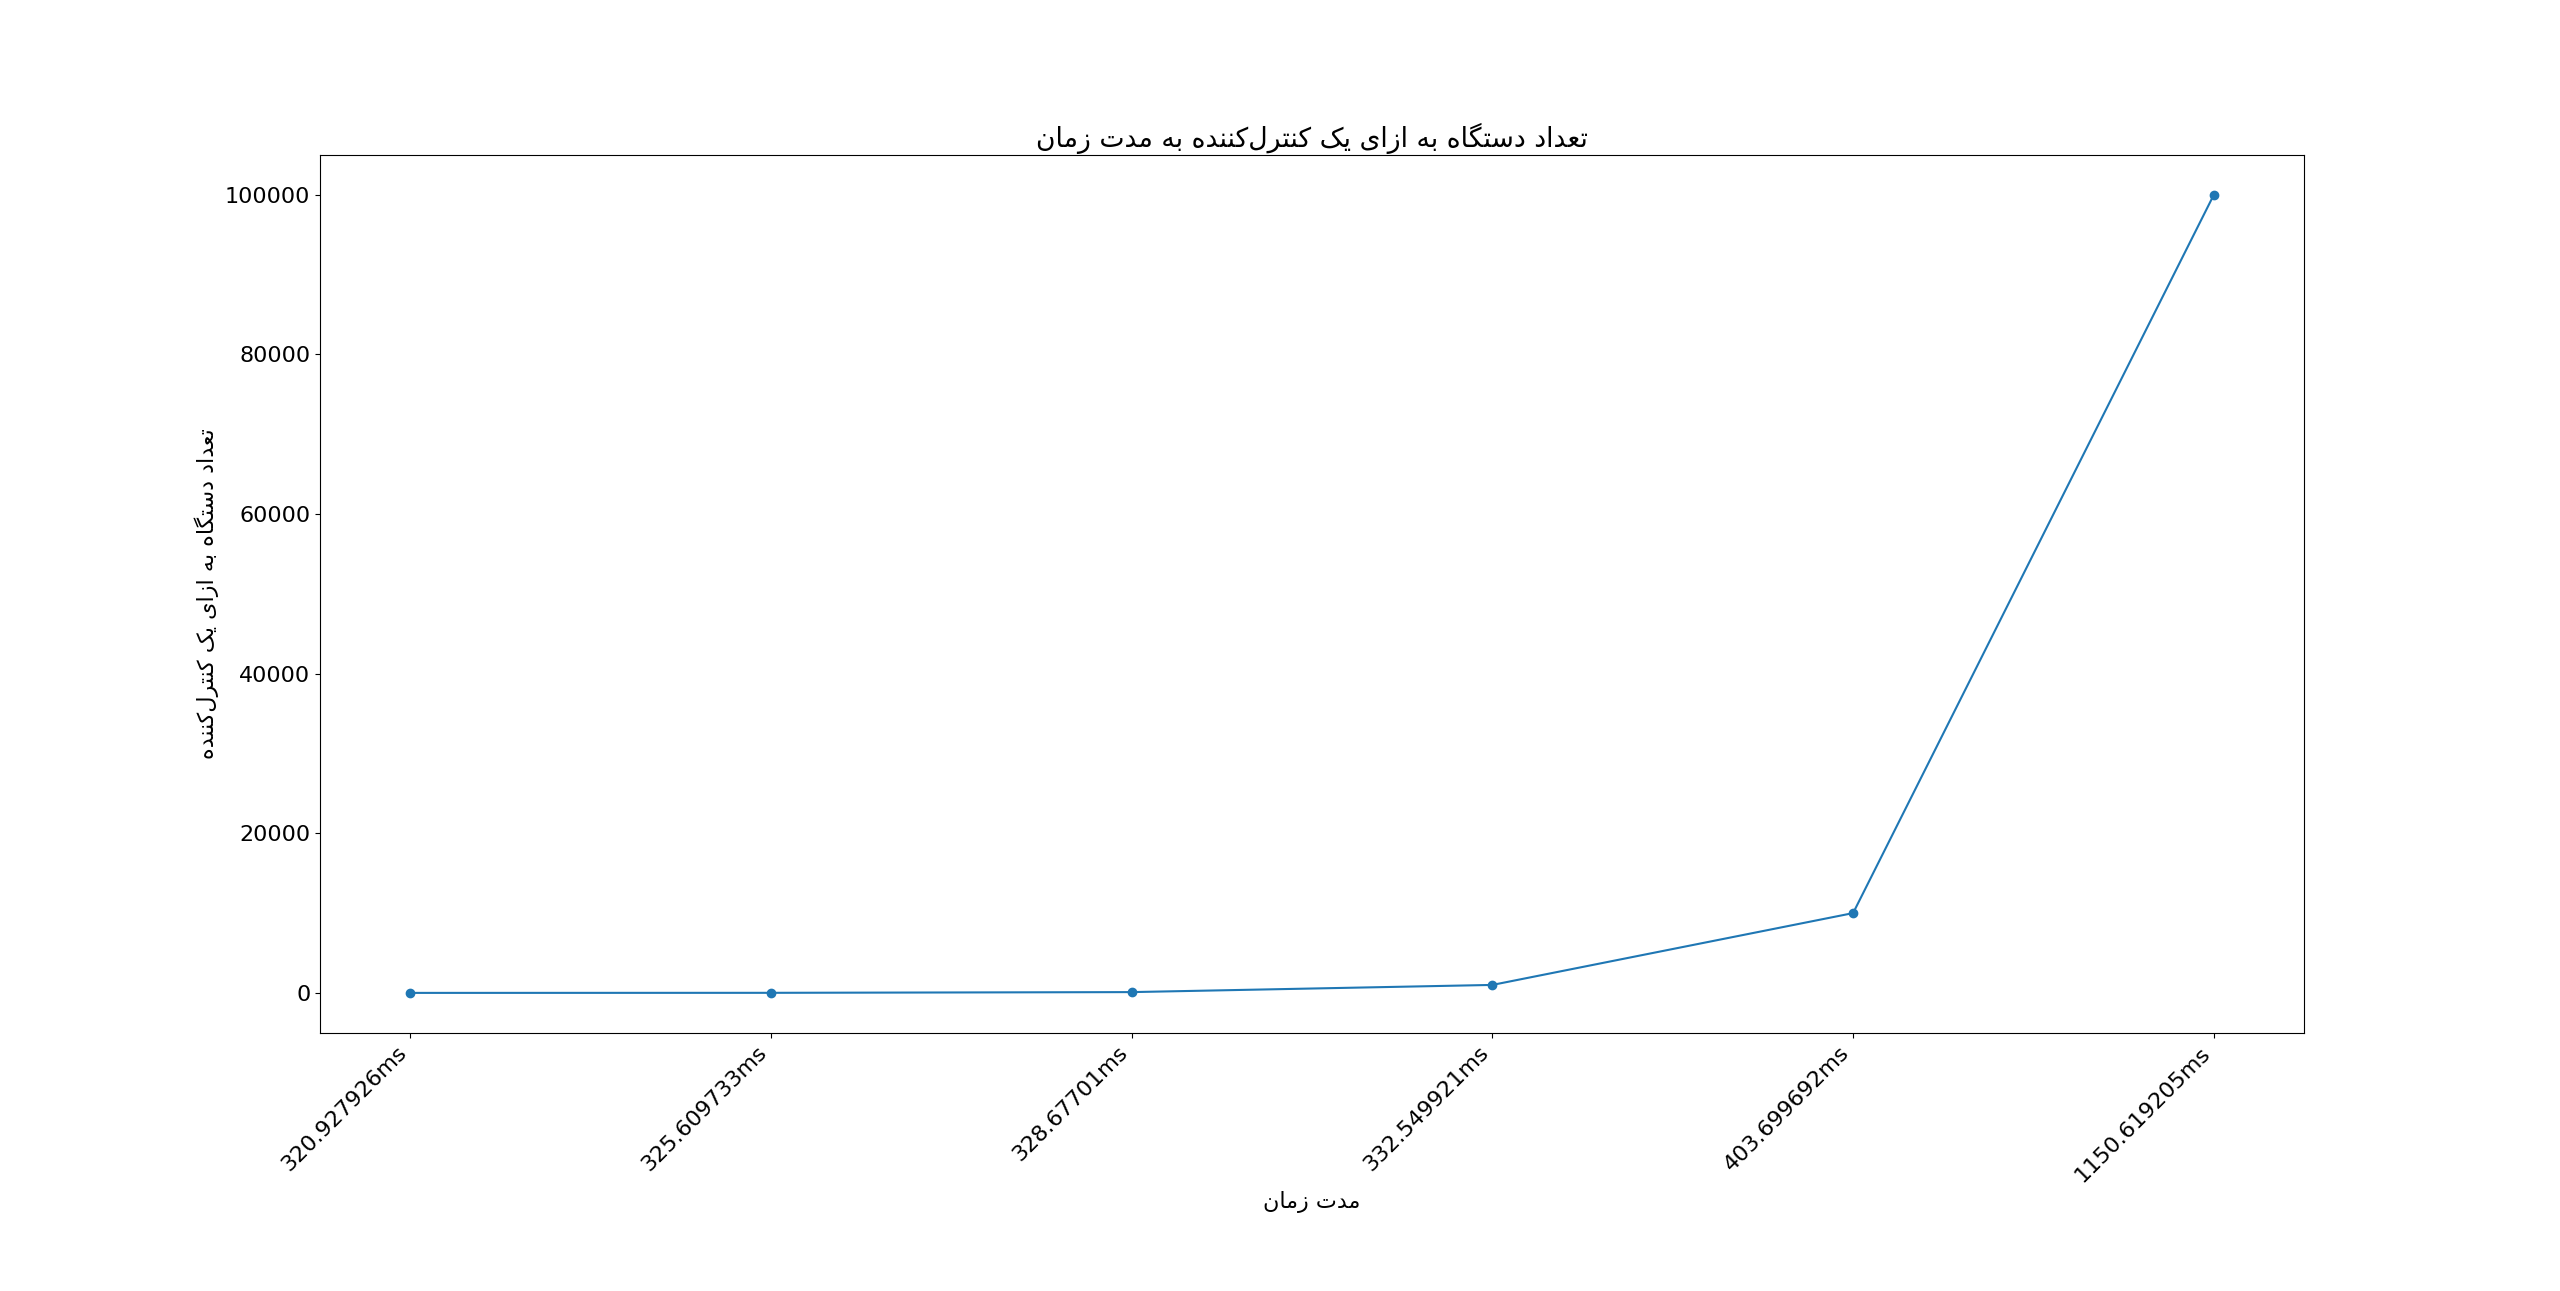
\includegraphics[width=0.9\textwidth]{figs/different_devices_plot.png}}
        \caption{نمودار تعداد کنترل‌کننده به مدت زمان}
        \label{fig:different_devices_plot}
    \end{figure}

    همانطور که مشاهده می‌شود با ده برابر کردن تعداد دستگاه‌ها در هر محله، مدت زمان سپری شده برای دریافت وضعیت همه‌ این دستگاه‌ها ده برابر نمی‌شود. بنابراین می‌توان انتظار گسترش بالایی از این روش داشت.
}


\section{
    بررسی توان تامین‌کننده با تعداد کنترل‌کننده دستگاه‌های اینترنت اشیاء مختلف
}
\label{sec:different_controllers}
\paragraph{}
{
    در این ارزیابی، تعداد دستگاه‌ به ازای هر کنترل‌کننده ثابت است اما تعداد کنترل‌کننده‌ها تغییر می‌کند. باید به این نکته توجه نمود که 
    با وجود ثبات تعداد دستگاه‌ها، به علت وجود یک دستگاه به ازای هر کنترل‌کننده، مجموع دستگاه‌ها برابر تعداد کنترل‌کننده‌ها خواهد بود.
    % Controllers,Time,Description
    % 1,316.631433ms,"Controllers: 1, DevicesPerController: 1, Duration: 5s"
    % 10,340.973697ms,"Controllers: 10, DevicesPerController: 1, Duration: 5s"
    % 100,632.569765ms,"Controllers: 100, DevicesPerController: 1, Duration: 5s"
    % 1000,3.487017751s,"Controllers: 1000, DevicesPerController: 1, Duration: 5s"
    % 10000,34.187790534s,"Controllers: 10000, DevicesPerController: 1, Duration: 1m0s"
    % 100000,45.409622456s,"Controllers: 100000, DevicesPerController: 1, Duration: 2m0s"
    \begin{table}[h]
        \centering
        \begin{tabular}{|c|c|}
        \hline
            تعداد کنترل‌کننده & مدت زمان                                                                                  \\ \hline
            ۱     &   \lr{۳۱۶.۶۳۱} میلی ثانیه                    \\ \hline
            ۱۰     &   \lr{۳۴۰.۹۷۳} میلی ثانیه                      \\ \hline
            ۱۰۰     &  \lr{۶۳۲.۵۶۹} میلی ثانیه                    \\ \hline
            ۱۰۰۰     &  \lr{۳۴۸۷.۰۱۷} میلی ثانیه                                                              \\ \hline
            ۱۰۰۰۰     & \lr{۳۴۱۸۷.۷۹۰} میلی ثانیه                  \\ \hline
            ۱۰۰۰۰۰     & \lr{۴۵۴۰۹.۶۲۲} میلی ثانیه  \\ \hline
        \end{tabular}
        \caption{جدول تعداد کنترل‌کننده به مدت زمان}
        \label{different_controllers_table}
    \end{table}

    \begin{figure}[H]
        \center{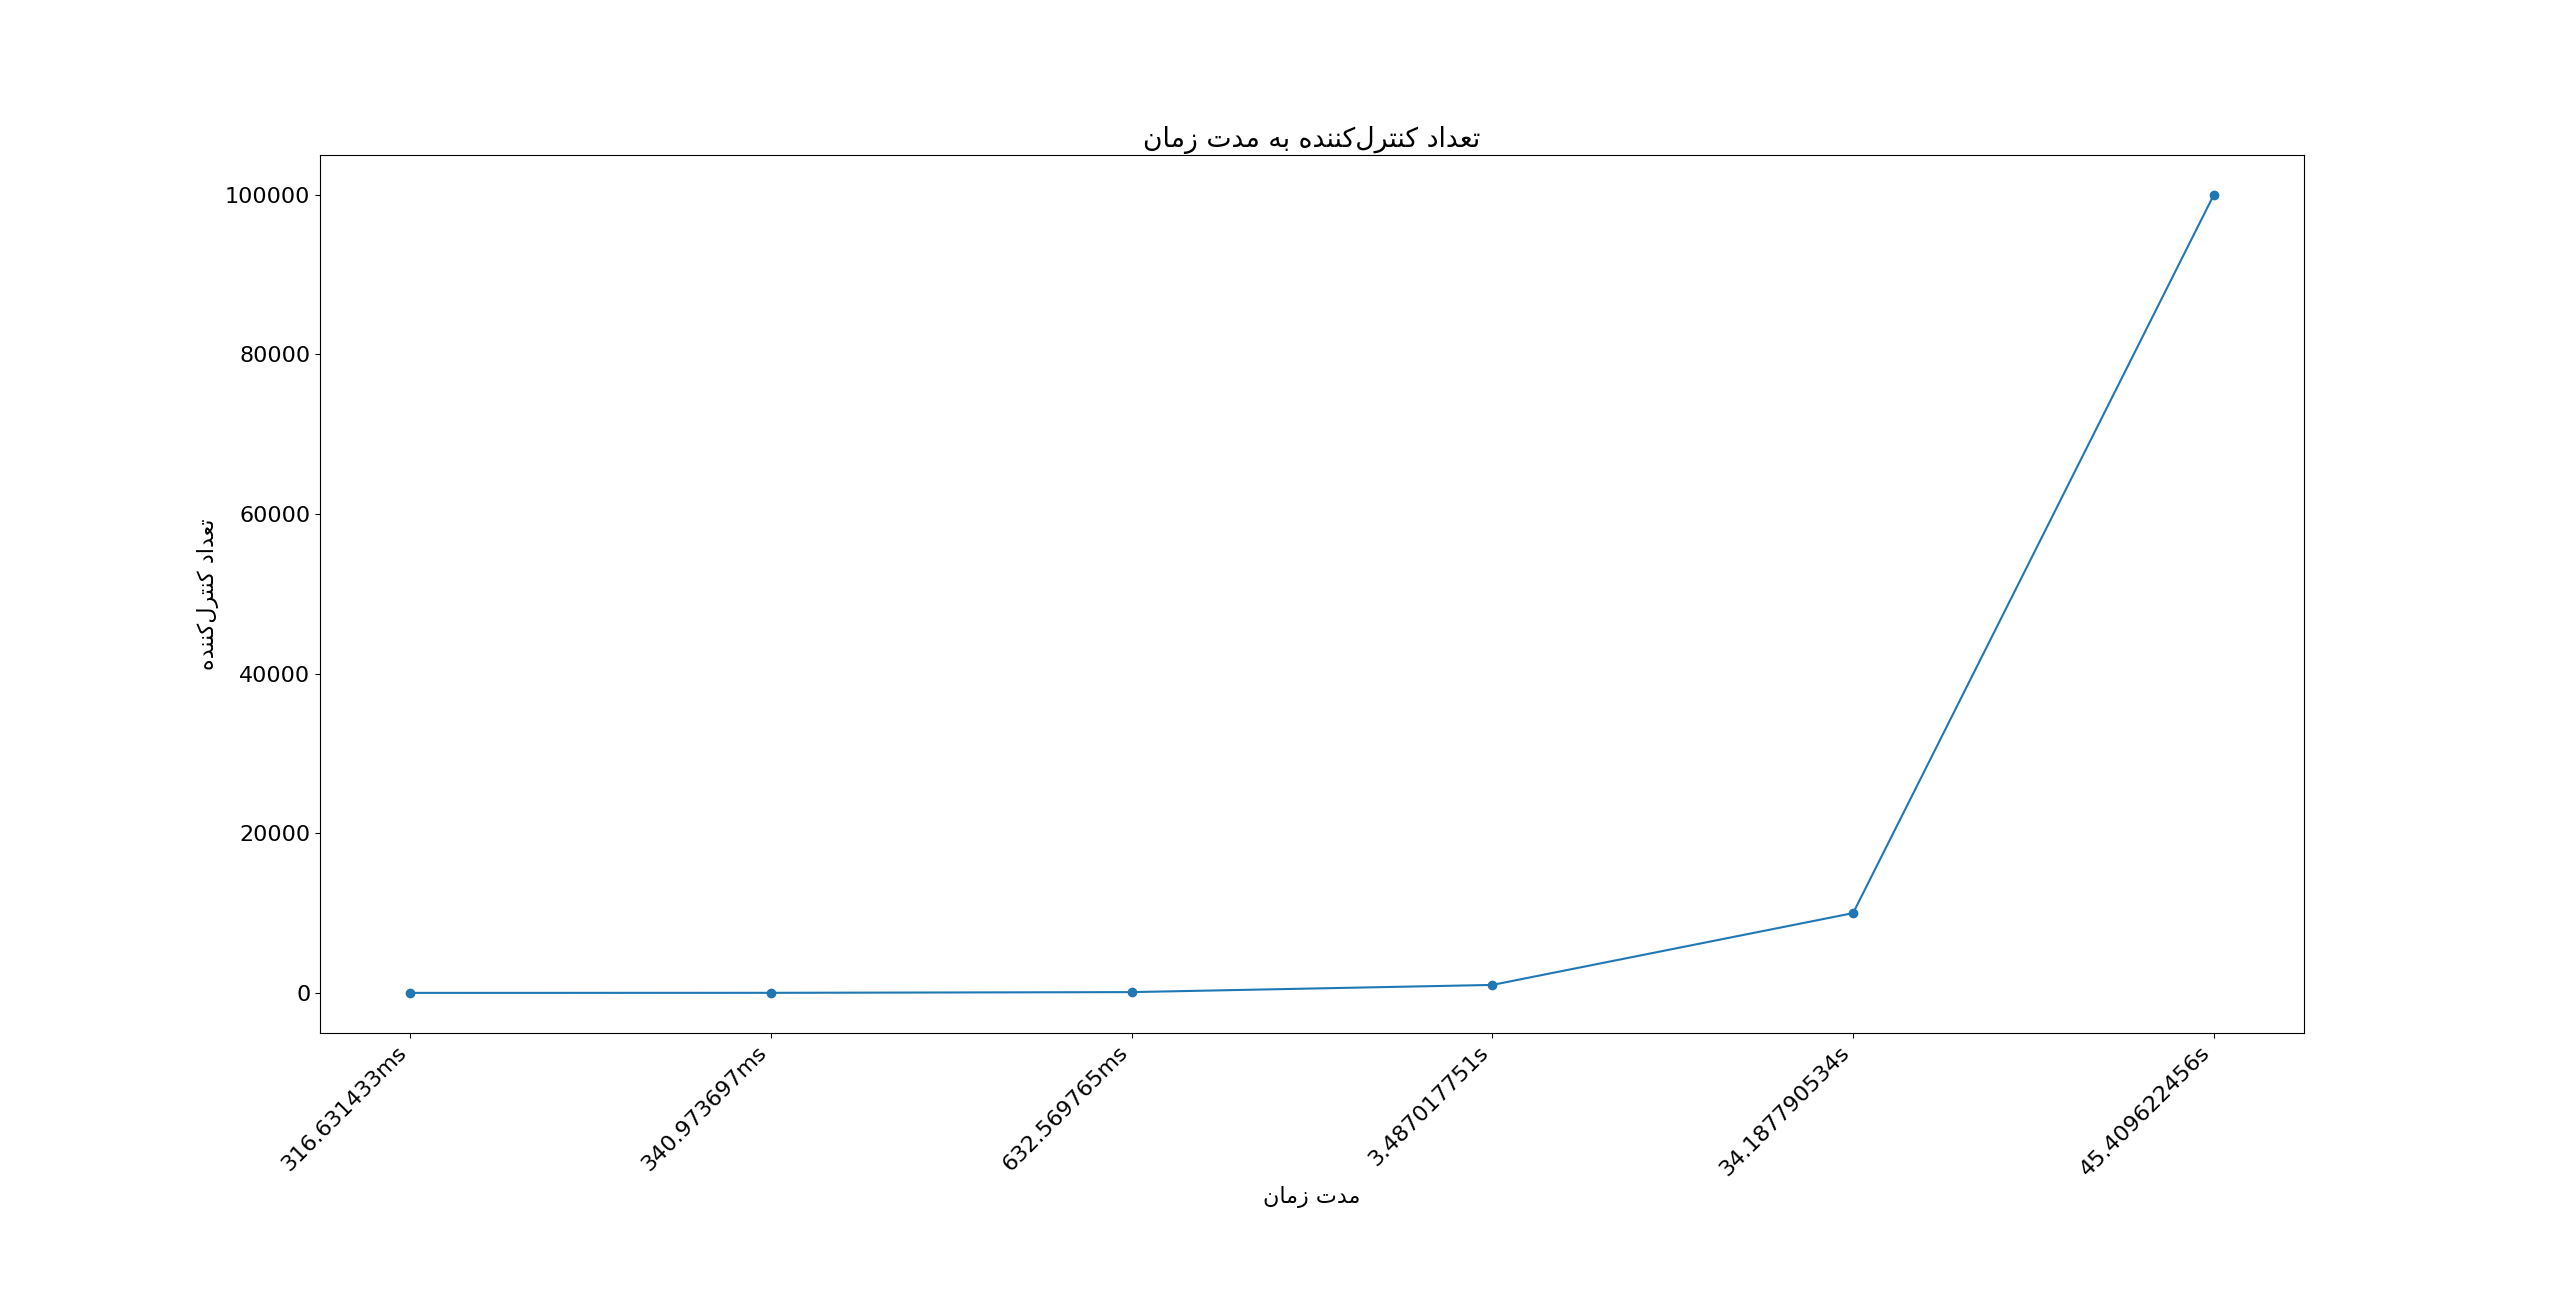
\includegraphics[width=0.9\textwidth]{figs/different_controllers_plot.png}}
        \caption{نمودار تعداد کنترل‌کننده به مدت زمان}
        \label{fig:different_controllers_plot}
    \end{figure}
}

\section{محدودیت‌های کوبرنیتز}
\label{sec:kubernetes_limitations}
\paragraph{}
{
    محدودیت اصلی این معماری، کوبرنیتز است. این سامانه تعداد پاد‌های محدودی را به ازای هر گره می‌تواند پشتیبانی کند (۲۵۶ پاد به ازای هر گره).
    البته که این تعداد برای پاد‌هایی هستند که کار محاسباتی انجام می‌دهند. بنابراین از نظر تئوری، این معماری می‌تواند تا 
    بی‌شمار دستگاه اینترنت‌ اشیاء به همراه کنترل‌کننده‌های آن‌ها را پایش و کنترل کند.
}

\section{جمع‌بندی}
\paragraph{}
{
    در این فصل دیدیم که معماری پیشنهادی توان کنترل تعداد زیادی دستگاه‌ اینترنت اشیاء را دارد و محدودیت اصلی از سوی کوبرنیتز
    اعمال می‌شود.
}